\documentclass{article}

% Language setting
% Replace `english' with e.g. `spanish' to change the document language
\usepackage[german]{babel}

% Set page size and margins
% Replace `letterpaper' with `a4paper' for UK/EU standard size
\usepackage[a4paper]{geometry}

% Useful packages
\usepackage{amsmath}
\usepackage{graphicx}
\usepackage[colorlinks=true, allcolors=blue]{hyperref}
\usepackage{multirow}

\title{Wirtschaft für Ingenieure}
\author{Asha Schwegler}

\begin{document}
\maketitle

\section{Grundprinzipien der Betriebswirtschaft}

\paragraph{Ökonomisches Prinzip:}
Spannungsverhältnis zwischen Unbegrenzte Bedürfnisse\\
und knappe Ressourcen.

\subsection{Gütereinteilung}
\paragraph{Güter werden aufgeteilt in:}

\begin{itemize}
\item Freie Güter
\item Wirtschaftliche Güter
\end{itemize}

\begin{figure}
\centering
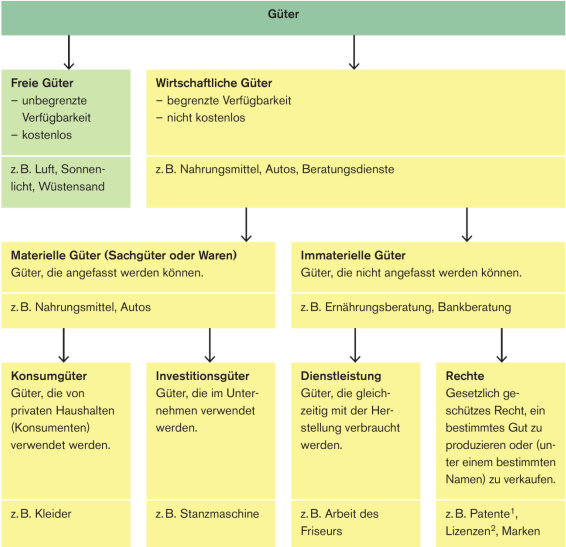
\includegraphics[width=0.3\textwidth]{Resources/Image/Guetereinteilung.png}
\caption{\label{fig:Guetereinteilung}Guetereinteilung.}
\end{figure}


\subsection{Markt}
Der Markt besteht aus Zusammenwirkung von Nachfrage und Angebot. \\
\subparagraph{Nachfrage:} Entsteht aus Bedarf, der wiederum aus Bedürfnisse entsteht.
\subparagraph{Angebot:} 
Entsteht aus der Herstellung


\subsection{Dreifache Unternehmensverantwortung}
\paragraph{Balance Akt zwischen:} 

\begin{itemize}
\item Gesamterhalt (Planet)
\item Selbsterhalt (Profit)
\item Miterhalt (People)
\end{itemize}

\begin{figure}
\centering
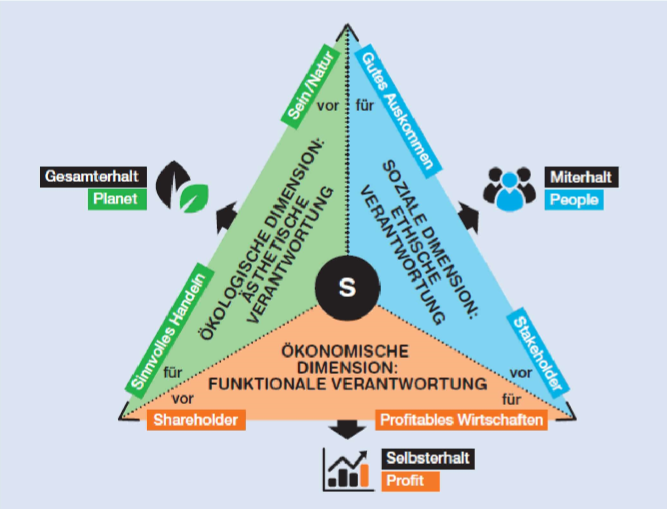
\includegraphics[width=0.3\textwidth]{Resources/Image/Dreifache Unternehmungsveratntwortung.png}
\caption{\label{fig:DreifacheUnternehmungsverantwortung}DreifacheUnternehmungsverantwortung.}
\end{figure}


\subsection{St. Galler Managementmodell}

\paragraph{SGMM: 3.Generation von 2002}

\begin{figure}
\centering
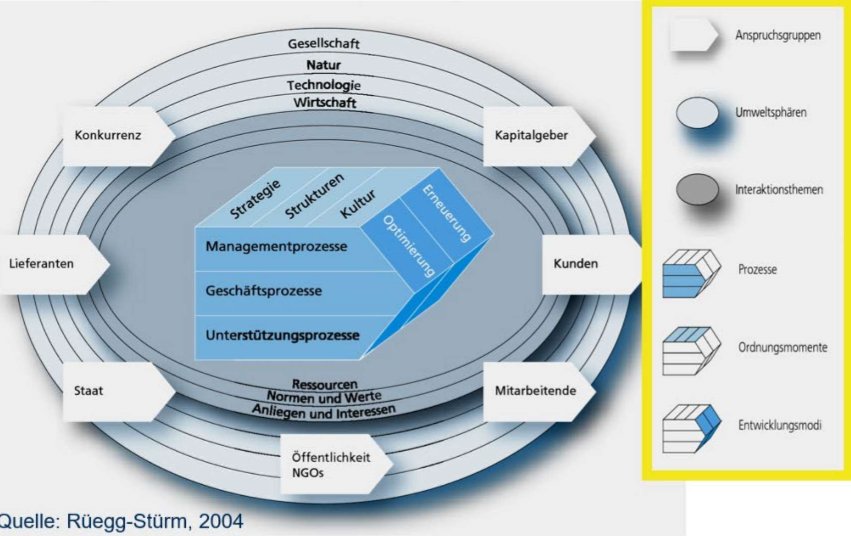
\includegraphics[width=0.3\textwidth]{Resources/Image/SGMM.png}
\caption{\label{fig:SGMM}SGMM.}
\end{figure}

\subsubsection{Umweltsphären}

\begin{tabular}{|l|l|}
\hline 
\rule[-1ex]{0pt}{2.5ex} \textbf{Umweltsphären} & \textbf{Beobachtungsbereiche} \\ 
\hline 
\rule[-1ex]{0pt}{2.5ex} Ökonomische Umwelt & Entwicklung Wirtschaft, Arbeitsmarkt, Teuerung, Wirtschaftsbeziehungen zum Ausland etc. \\ 
\hline 
\rule[-1ex]{0pt}{2.5ex} Technologische Umwelt & Produktionsverfahren, Materialien, Transport- und Kommunikationsmittel etc. \\ 
\hline 
\rule[-1ex]{0pt}{2.5ex} Soziale Umwelt & Politische und gesellschaftliche Trends, Wohlbefinden der einzelnen Menschen etc. \\ 
\hline 
\rule[-1ex]{0pt}{2.5ex} Ökologische Umwelt & Rohstoffe, Energie, Klima, Abfälle, etc. \\ 
\hline 
\end{tabular} 


\subsubsection{Anspruchsgruppen / Stakeholder}
\begin{enumerate}
\item Sind von der Tätitigkeit der Unternehmen betroffen. 
\item Haben Erwartungen und Ansprüche.
\end{enumerate}
 

\subparagraph{Machtausübung Primär:}
\begin{itemize}
\item faktische
\item vertragliche
\item gesetzliche
\item oder normative Grundlagen
\end{itemize}


\subparagraph{Sanktionsgrundlage Sekundär:}
\begin{itemize}
\item gesellschaftspolitische
\item witschaftsethische Konventionen
\end{itemize}

\begin{figure}
\centering
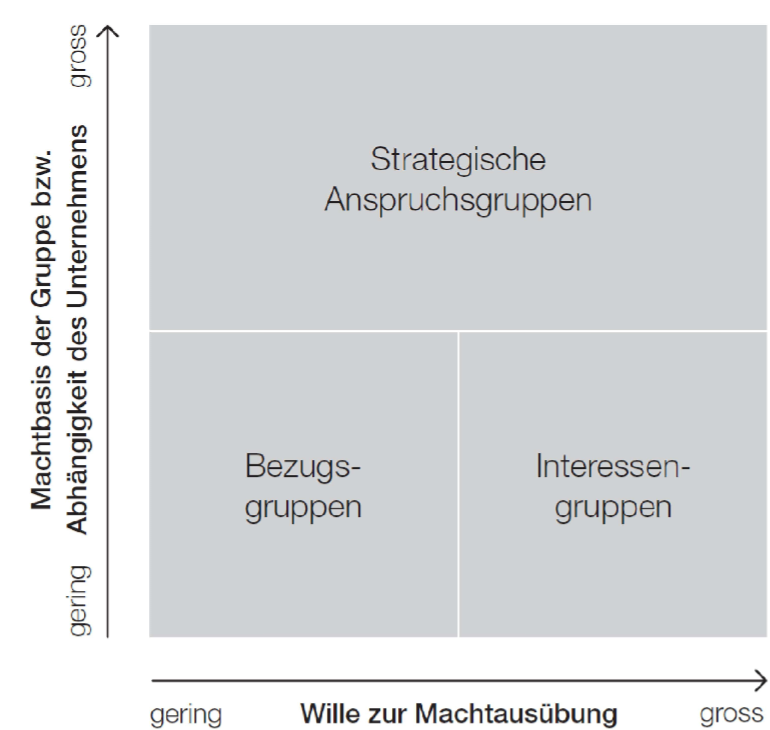
\includegraphics[width=0.3\textwidth]{Resources/Image/MachtausuebungStakeholder.png}
\caption{\label{fig:MachtausuebungStakeholder}MachtausuebungStakeholder.}
\end{figure}

\subsubsection{Interaktionsthemen}

\paragraph{Interaktionsthemenanalyse:}
\begin{enumerate}
\item Bestimmte Anspruchsgruppe
\item Anliegen und Interessen aufzeigen
\item Vorliegende Normen und Werte prüfen
\end{enumerate}

\paragraph{Ressourcen:}
\begin{enumerate}
\item Arbeit, Boden, Kapital, Wissen
\item Marke, Reputation, Image, Vertrauen
\end{enumerate}


\paragraph{Vorgehen:}

\subparagraph{1. Sachverhalt:}
\begin{itemize}
\item Welche Ressource des Unternehmens ist betroffen
\item In Welche Umweltsphäre spielt sich Sachverhalt ab
\end{itemize}

\subparagraph{2. Welche Anspruchsgruppe:}
\begin{itemize}
\item Anliegen / Ziele
\item Interessen
\item Normen (Gesetze und Regeln)
\item Werte
\end{itemize}

\subparagraph{3. Aus Unternehmenssicht:}
\begin{itemize}
\item Gefahren
\item Reaktionsmöglichkeiten
\end{itemize}

\begin{figure}
\centering
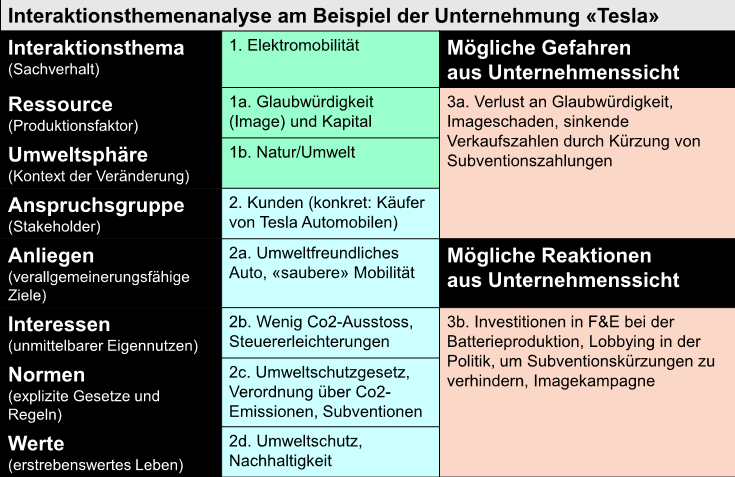
\includegraphics[width=0.3\textwidth]{Resources/Image/Interaktionsthemenanalyse.png}
\caption{\label{fig:Interaktionsthemenanalyse}Interaktionsthemenanalyse.}
\end{figure}


\section{Strategie}
\subparagraph{Einordnung:}
\begin{figure}
\centering
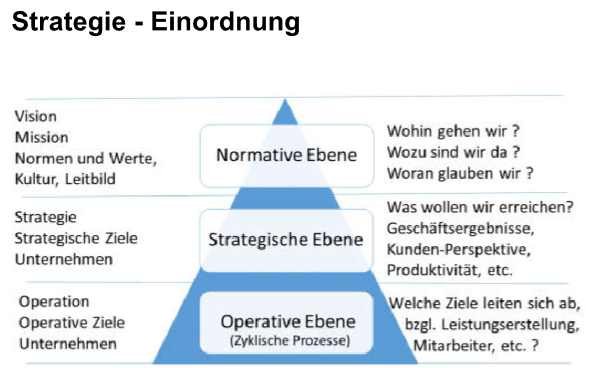
\includegraphics[width=0.3\textwidth]{Resources/Image/StrategieEinordnung.png}
\caption{\label{fig:StrategieEinordnung}StrategieEinordnung.}
\end{figure}

\subparagraph{für Management-Entscheide:}
\begin{figure}
\centering
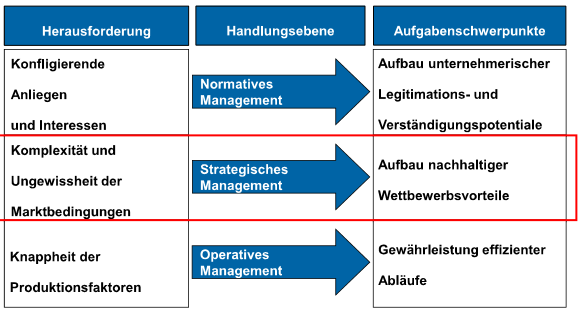
\includegraphics[width=0.3\textwidth]{Resources/Image/ManagementEntscheide.png}
\caption{\label{fig:ManagementEntscheide}ManagementEntscheide.}
\end{figure}


\subsection{Strategiefindungsprozess}
\paragraph{In vier Schritten:}
\begin{enumerate}
\item Strategische Analyse
\item Strategische Planung
\item Strategische Umsetzung
\item Strategische Messung
\end{enumerate}

\subsection{Die strategische Analyse}
\subparagraph{Drei Modellen:}
\begin{itemize}
\item SWOT-Analyse
\item PESTEL-Analyse
\item 5-Forces Modell von Porter
\end{itemize}

\subparagraph{Faktoren, die Analyse beeinflussen}
\begin{figure}
\centering
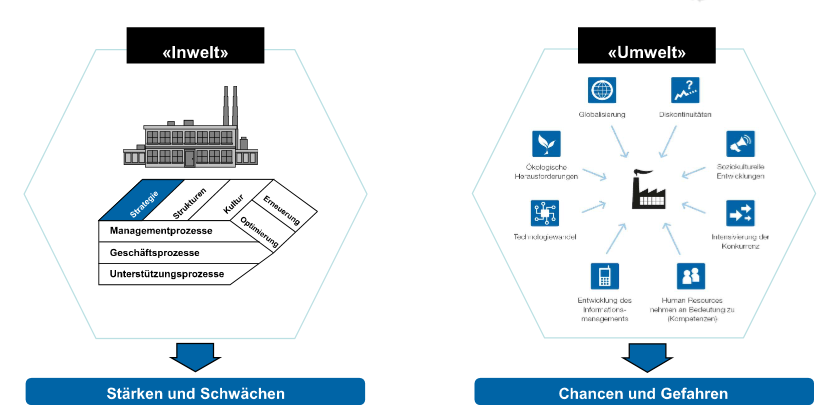
\includegraphics[width=0.3\textwidth]{Resources/Image/FaktorenEinfluss.png}
\caption{\label{fig:FaktorenEinfluss}FaktorenEinfluss.}
\end{figure}

\subsubsection{SWOT-Analyse:}
\begin{figure}
\centering
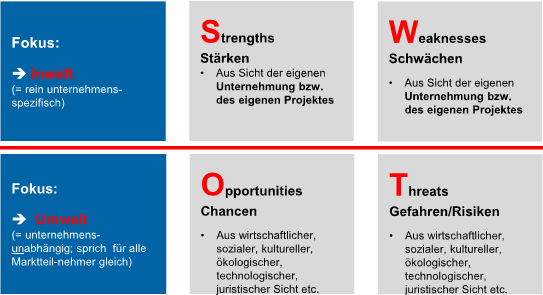
\includegraphics[width=0.3\textwidth]{Resources/Image/SwotAnalyse.png}
\caption{\label{fig:SwotAnalyse}SwotAnalyse.}
\end{figure}

\subparagraph{Kern-Kompetenzen:}

Kompetenz als Wettbewerbsvorteil
\begin{itemize}
\item Wertvoll
\item Selten
\item Nicht oder schwer imitierbar
\item Nicht substituierbar
\end{itemize}


\paragraph{Unternehmensanalyse Beispiel Easyjet \\ \\}

\begin{tabular}{|l|c|}
\hline
\rule[-1ex]{0pt}{2.5ex} 
\textbf{Strenghts} & \textbf{Weaknesses} \\ 
\hline 
\rule[-1ex]{0pt}{2.5ex}
Moderne Flugzeuge mit tiefen Betriebskosten & Keine Interkontinentalflüge \\ 
\hline 
\rule[-1ex]{0pt}{2.5ex}
Ersten Fluggesellschaften,Internetplattform zum Buchen & Gewisse (teure)Flughäfen  nicht Streckennetz \\ 
\hline
\rule[-1ex]{0pt}{2.5ex} 
Einheitliches Angebot (Bloss Ecenomy Class etc) &  \\ 
\hline
\rule[-1ex]{0pt}{2.5ex}
\end{tabular} \\ \\


\begin{tabular}{|l|l|}
\hline 
\rule[-1ex]{0pt}{2.5ex}
\textbf{Opportunities} & \textbf{Threats} \\ 
\hline 
\rule[-1ex]{0pt}{2.5ex} Wetter(Schlecht in CH zu Gut Ausland) & Covid-19 Reisebeschränkungen \\ 
\hline 
\rule[-1ex]{0pt}{2.5ex} Trend Wochenend Städtereisen & Verteuerung Treibstoffkosten \\ 
\hline 
\rule[-1ex]{0pt}{2.5ex} Grössere Flugzeuge & Höhere Flughafentaxen \\ 
\hline 
\rule[-1ex]{0pt}{2.5ex} Steigender Wohlstand & Verlängerung Nachtflugsperre europ.Flughafen \\ 
\hline 
\rule[-1ex]{0pt}{2.5ex}  & Neue Billig-Airlines \\ 
\hline 
\end{tabular} 


\paragraph{Die vier abgeleiteten Grundstrategieansätze: \\}
\begin{figure}
\centering
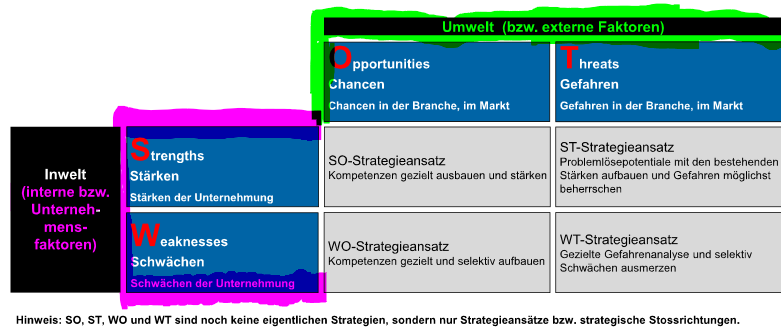
\includegraphics[width=0.3\textwidth]{Resources/Image/GrundstrategieAnsaetze.png}
\caption{\label{fig:GrundstrategieAnsaetze}GrundstrategieAnsaetze.}
\end{figure}


\subsubsection{PESTEL-Analyse}

Untersucht den Einfluss der sechs \textbf{externen} Umweltfaktoren \\
\begin{figure}
\centering
\includegraphics[width=0.3\textwidth]{Resources/Image/Pestelanalyse.png}
\caption{\label{fig:Pestelanalyse}Pestelanalyse.}
\end{figure}




\subsubsection{5 Kräfte Modell von Porter}

Untersucht den Markt. \\



























\bibliographystyle{alpha}
\bibliography{sample}

\end{document}